For the implementation of the model we used MATLAB. In order to keep the code readable as the project grows, we split the main functionalities into different files.
\begin{figure}[H]
	\centering
	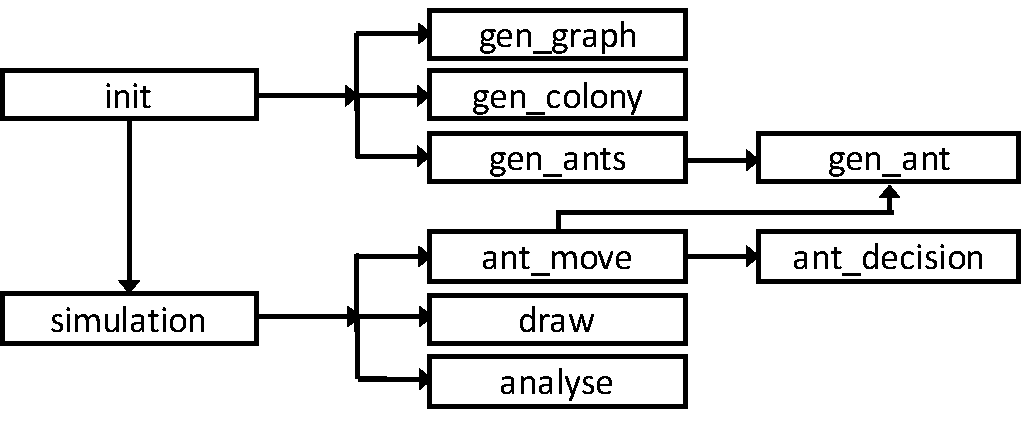
\includegraphics[scale=0.5]{Dependencies.pdf}
	\caption{Dependencies of the different MATLAB scripts. The arrows indicate calls of functions}
\end{figure}
The only executable file is \textit{init.m}. It defines all global variables like the mean lifetime of pheromones, the number of ants and the parameters of the simulation. All the objects, which are important to the simulation are also created in this file. This is done by a call of \textit{gen\_sources}, \textit{gen\_colonies}, \textit{gen\_graph} and \textit{gen\_ants}. The generated structures are then fed into the \textit{simulation} script, where a simulation loop is implemented and the position of the ants is updated by \textit{ant\_move} for the specified number of iterations. The relevant data is then stored and processed by the \textit{analyze} function. In the end the result of the analysis is visualized by the \textit{draw} function.
\subsection{Environment}
The environment of the model is mainly defined by the graph on which the simulation runs. 
The graph itself is generated by the python script \textit{graph\_generator}. It constructs the nodes and weighted edges of the graph. Furthermore it determines the differnt types of nodes for the network. The edges are chosen probabilisticly, such that the probability of the edge being in the graph decreases exponentially with the distance of the edge. This implies, that nodes, which are located closer together have a higher probability to form a connection. This results in a graph which is closer to a real network (such as the rail network).

In the \textit{init} script, the graph gets initialized. There are two different types of nodes in the network. The source nodes and traffic nodes.
Each source node is the start of a colony. However the members of a colony do not see their own starting node as a food source (they can not get their food from their starting node). But the starting nodes of other colonies are seen as food sources. Afterwards the ants are generated and distributed equally among the colonies. 

Finally the global paramaters are set for the simulation. The paramaters were chosen by us empirically. Each colony gets 200 ants, which is enough to build sophisticated paths and is computationally feasable. The mean live time of phermons is set to 30, this ensures that ants can explore most of the graph and the phermons are still there to enforce the probability when they encounter the path a second time. The food limit per source was set to 200 as well to match the number of ants in the system. However the sources differ in their food regeneration rate. The simulation itself runs 1000 timesteps, where each ant moves a distance of 1 per timestep. This has proven to be enough time to stabilize the system.

\subsubsection{Rail network}
For the second part of our goal, to maximize the productivity in the Swiss rail network we have to be able to utilize the graph of this network. We got the data to construct this graph from a graphic outlining all the far distance connection of the SBB \citep{SbbStats2}. We chose to select the colonies to be the train stations with the most visitors per day \citep{SbbStats1}. The weight of the edges is not given by the physical distance, but by the time it takes to travel from one node to the other by a direct connection (based on the SBB time table)\citep{SbbStats3}. To draw the graph we used the Swiss coordinate system and normalized it, so that Geneva is the origin. In the drawn version the edges represent geographical distance.

\begin{figure}[H]
	\centering
	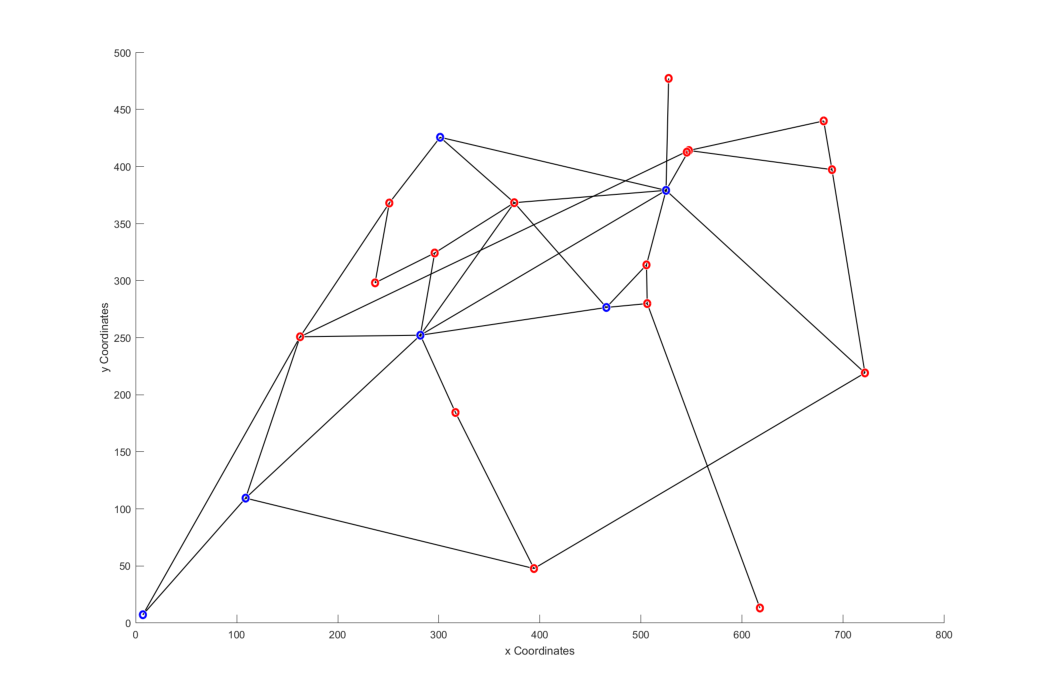
\includegraphics[scale=0.8]{sbbEmpty.pdf}
	\caption{Graphic of the Swiss Rail Graph. The blue circles indicate sources (and colonies), the red circles represent traffic nodes. The units of the x- and y-axis are from the Swiss coordinate system}
\end{figure}

\subsection{Ant behaviour}
The movement and decision of the ants is based on the model described in chapter \ref{modeldesc}. The script responsible for the update of the position at every time step is called \textit{ant\_move}. There the next position of the ant on the graph is determined. The ant has a variable to store the progress on the edge. As soon, as this progress reaches the weight of the edge a node has been reached. If the node is a food source, different from the starting point the ant will bring some of the food back to the colony. By doing so the food source will experience a devaluation. The ant follows exactly the same path back to its nest, that it took on the way to the source. On the way back it will deposit pheromones, with an intensity depending on the quality of the found food source. The pheromones are saved in a variable of the edges. Each colony has their own pheromones, the decision of the ant is not affected by the trail laying of the ants from other colonies.
If the found node is a traffic node, then the ant has to make a decision between the n adjacent paths. This decision happens in the \textit{ant\_decision} function. As seen in formula \ref{multiDecisions} the decision depends on the concentration of pheromones on the path. This concentration is calculated by
\begin{equation}
c = \frac{pheromones}{weight}
\end{equation}
Where weight is the length of an edge. The ant is free to choose from all the edges on the node, except for the one it used to get there.
However this freedom presents another problematic. Because the ant is free to choose between all the edges it is allowed to walk in circles. Those cycles would then be reinforced by the trail laying on the way back. To solve this we still allow the ants to walk in circles, but when they do the circle will be removed from the path vector, which is used to find the way back to the nest.
The U-turns are implemented exactly as described in equation \ref{UTurn}. At every time step this probability is calculated. With this probability a U-turn happens and the ant walks back to the last visited node. 
\subsection{Ant reallocation}
As described in the introduction chapter, the goal is to maximise the productivity of the network by reallocating ants to other colonies. In the following the implementation of the two strategies is explained.
\subsubsection{Local reallocation}
Remember from chapter \ref{intro}, that the productivity of an colony is calculated by the total food, brought back to the colony per time. Hence the productivity of a single ant of a colony is calculated by dividing the productivity of the colony by the number of corresponding ants. Now when the ant finds a colony it has a probability of staying there and work for them (Formula \ref{localRealloc})
\begin{equation} \label{localRealloc}
P = max(0,\frac{Prod_{ant}-Prod_{new}}{Prod_{ant}+Prod_{new}})
\end{equation}
P describes the probability of staying at the new colony, $Prod_{ant}$ stands for the productivity of the arriving ant and $Prod_{new}$ for the productivity of the ants at the new colony.
\subsubsection{Global reallocation}
In contrary to the local approach, the ants do not have to walk to their new home in the global solution. Instead the reallocation happens, when the ant arrives at its own nest. If the productivity of that ant is lower, then the global average productivity, The ant can be transferred to a new colony. To determine whether the ant is moved a modification to equation \ref{localRealloc} is made, where $prod_{new}$ is replaced by the global average productivity. If moved the target colony is then determined by chance out of all the colonies, which perform better then average.
If an ant is transferred, it happens instantly. At the next time step the ant will be part of the new colony.